\documentclass{article}
\usepackage{graphicx} % Required for inserting images
\usepackage[margin=3cm]{geometry} % Adjust the margin as needed
\usepackage{tabularx}
\usepackage[italian]{babel}
\usepackage{float}
\usepackage{hyperref}
\usepackage{caption}
\usepackage{subcaption}
\usepackage{listings}
\usepackage{amsmath}
\usepackage{xcolor}
\usepackage[table]{xcolor}

% Colori stile Visual Studio
\definecolor{vsblue}{RGB}{0, 0, 255}
\definecolor{vsgreen}{RGB}{0, 128, 0}
\definecolor{vsred}{RGB}{163, 21, 21}
\definecolor{vspurple}{RGB}{128, 0, 128}
\definecolor{vsgray}{RGB}{128, 128, 128}
\definecolor{vsbackground}{RGB}{248, 248, 248}
\definecolor{vsborder}{RGB}{220, 220, 220}

\lstdefinestyle{visualstudio}{language=C++,
    backgroundcolor=\color{vsbackground},
    basicstyle=\ttfamily\footnotesize,
    keywordstyle=\color{vsblue},
    commentstyle=\color{vsgreen},
    stringstyle=\color{vsred},
    identifierstyle=\color{black},
    numberstyle=\tiny\color{vsgray},
    numbers=left,
    numbersep=10pt,
    frame=single,
    rulecolor=\color{vsborder},
    framerule=0.5pt,
    breaklines=true,
    breakatwhitespace=false,
    columns=fullflexible,
    keepspaces=true,
    showstringspaces=false,
    tabsize=4,
    captionpos=b
}

\newcommand{\code}[1]{\texttt{#1}}

\title{Random Maze Solver \\ \vspace{0.5cm} {Parallelizzazione con OpenMP della risoluzione concorrente di un labirinto}}
\author{Lorenzo Cappellini}
\date{Parallel Computing - A.A. 2025/2026}

\begin{document}

\maketitle

\newpage

\tableofcontents

\newpage
\section{Introduzione}

\subsection{Obiettivo}
Il progetto è stato sviluppato per l'assignment del corso di Parallel Computing, il quale richiede l'implementazione di un programma che sfrutti almeno uno degli approcci di parallelizzazione o vettorizzazione presentati durante il corso (OpenMP, vettorizzazione SIMD, CUDA), a partire da una versione sequenziale dello stesso algoritmo, corredata da un'analisi delle performance in termini di \textit{speedup}.
\\

\noindent Il problema scelto è il \textbf{Random Maze Solver}: dato un labirinto, l'obiettivo è individuare l'uscita simulando il movimento casuale di una "particella". Questa parte da una posizione iniziale all'interno del labirinto e si muove casualmente tra le celle; quando incontra un muro, la particella rimbalza.\\
Per aumentare la probabilità di individuare rapidamente l'uscita, vengono "lanciate" simultaneamente un numero elevato di particelle, ciascuna delle quali segue il proprio percorso. La simulazione termina quando la prima particella riesce a uscire dal labirinto. A questo punto, il percorso seguito dalla particella vincente viene ricostruito tramite \textit{backtracking}, permettendo di individuare il cammino che conduce all'uscita.\\
\\

\noindent Il codice sorgente è disponibile su Github al seguente indirizzo:\\
\href{https://github.com/lcappellini/RandomMazeSolver}{https://github.com/lcappellini/RandomMazeSolver}.

\subsection{Approcci utilizzati}
Dato che \textbf{ogni particella è indipendente} dall'altra, il problema si presta particolarmente alla parallelizzazione mediante \textbf{OpenMP}: ogni thread può occuparsi dell'avanzamento di una particella (o più) in modo indipendente.\\
L'unica forma di \textbf{sincronizzazione} necessaria riguarda l'individuazione della prima particella che raggiunge l'uscita e la conseguente terminazione di tutti i restanti thread.
\\

\noindent Il carico di lavoro non è descritto da un'unica variabile ma da \textbf{due grandezze distinte}:
\begin{itemize}
    \item il \textbf{numero di particelle} lanciate, che determina quanti tentativi indipendenti di ricerca casuale vengono effettuati.\\
    Più particelle $\Rightarrow$ più probabilità di trovare un percorso migliore $\Rightarrow$ minor tempo di esecuzione;
    \item il \textbf{numero di thread} su cui tali particelle vengono effettivamente distribuite ed eseguite in parallelo.\\
    Più thread $\Rightarrow$ più parallelismo $\Rightarrow$ minor tempo per far avanzare le particelle.
\end{itemize}

\noindent Per semplicità di gestione e implementazione non è specificato il numero totale di particelle, ma il numero di particelle che ogni thread lancia.

\begin{figure}[H]
    \centering
    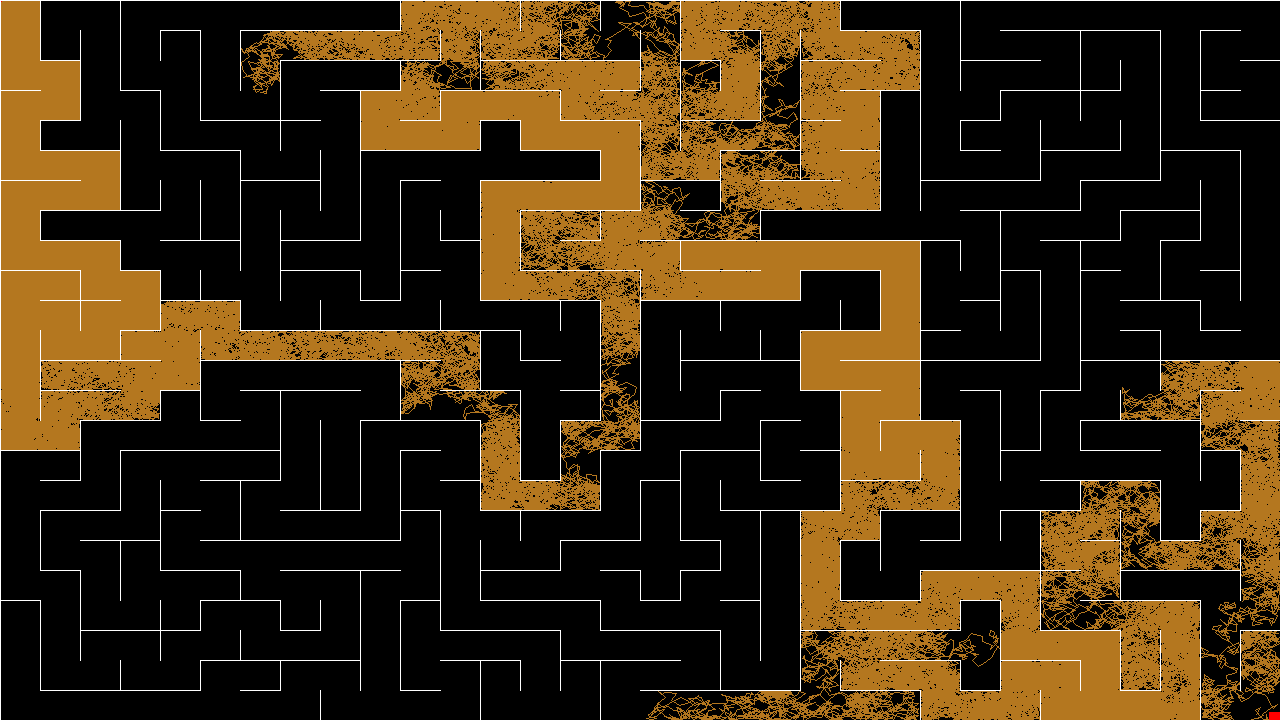
\includegraphics[width=0.9\textwidth]{Graphs/maze.png}
    \caption{Immagine del labirinto con una particella che si muove randomicamente dalla partenza (in alto a sinistra) fino a raggiungere l'uscita (in basso a destra) in $350000$ steps (caso ottimo)}
    \label{fig:maze_picture}
\end{figure}

\begin{figure}[H]
    \centering
    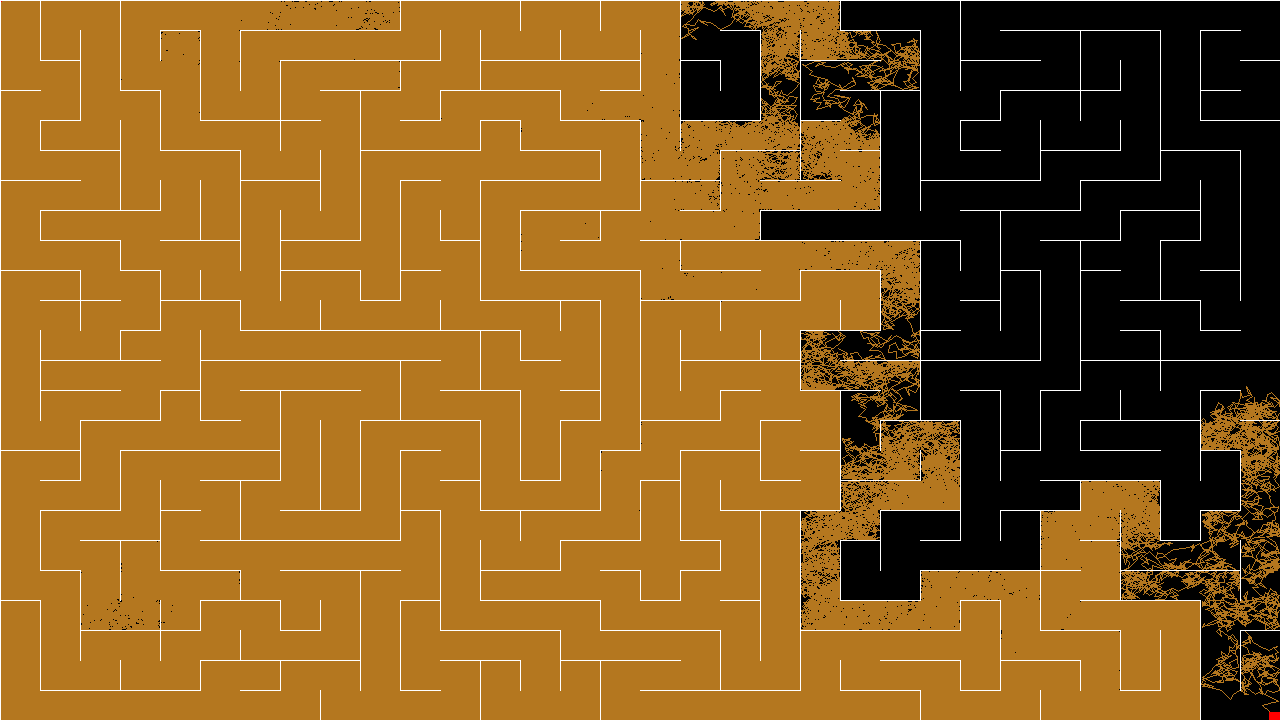
\includegraphics[width=0.9\textwidth]{Graphs/maze2.png}
    \caption{Immagine del labirinto con una particella che si muove randomicamente dalla partenza (in alto a sinistra) fino a raggiungere l'uscita (in basso a destra) in $5$ milioni di steps (caso pessimo)}
    \label{fig:maze_picture2}
\end{figure}

\newpage

\section{Architettura e implementazione}

\subsection{Flusso del programma}
Per ciascuna coppia (numero di particelle per thread $p$, numero di thread $n$), il programma:
\begin{enumerate}
    \item genera lo stesso labirinto di partenza, riutilizzato per tutte le misurazioni;
    \item avvia $n$ thread (tramite le direttive OpenMP e \code{num\_threads(n)}), ognuno dei quali lancia $p$ particelle indipendenti $\Rightarrow$ totale $p*n$ particelle;
    \item avanza le particelle con step random ottenuti dagli \code{StepGenerator}, in un range $(-step, +step)$ per le due coordinate x e y;
    \item appena una particella arriva all'uscita (entra nella regione di arrivo), misura il tempo trascorso tramite \code{std::chrono::high\_resolution\_clock}, e ritorna anche il numero di iterazioni impiegate;
    \item ripete la misurazione più volte per ciascuna coppia $(p, n)$;
    \item salva le misurazioni effettuate in un file \code{.csv}.
\end{enumerate}
La griglia di configurazioni testate copre $p \in {1, \dots, 20}$ e $n \in {1, \dots, 16}$, per un totale di $320$ configurazioni distinte, ciascuna ripetuta $100$ volte.

\subsection{Classi}
Per modellare il problema sono state create varie classi:

\begin{itemize}
    \item \textbf{\code{Point}}: struttura dati elementare che rappresenta un punto geometrico, con coordinate $(x, y)$.
    \item \textbf{\code{Rect}}: rappresenta un rettangolo geometrico, utilizzato per delimitare la regione di arrivo (uscita del labirinto); tramite il metodo \code{inside(Point\&)} è possibile verificare se un \code{Point} è al suo interno.
    \item \textbf{\code{Path}}: identifica il percorso della particella tramite un vector di \code{Point}.
    \item \textbf{\code{StepGenerator}}: implementa un generatore di numeri casuali (RNG) secondo una distribuzione uniforme in un range specificato.
    \item \textbf{\code{Maze}}: rappresenta il labirinto, suddiviso per semplicità in celle rettangolari, ciascuna delle quali specifica l'eventuale presenza di un muro nei quattro lati. Internamente si occupa di:
    \begin{itemize}
        \item generare il labirinto randomicamente tramite l'algoritmo di \textit{Recursive Backtracking};
        \item validare i movimenti delle particelle calcolando gli eventuali rimbalzi sui muri;
        \item disegnare il labirinto e i percorsi trovati su un'immagine (tramite la libreria \code{OpenCV});
    \end{itemize}
    \item \textbf{\code{MazeSolver}}: implementa la logica di risoluzione vera e propria, facendo avanzare le particelle con movimenti rettilinei di lunghezza casuale finché uno di essi non raggiunge la regione di arrivo. Internamente suddivide il lavoro sul numero specificato di thread.
\end{itemize}

\newpage

\subsection{Generazione del labirinto}
Il labirinto viene generato, in modo sequenziale, tramite l'algoritmo di \textbf{Recursive Backtracking}: partendo dalla cella $(0,0)$, l'algoritmo visita ricorsivamente le celle adiacenti non ancora visitate in ordine casuale, rimuovendo il muro condiviso tra la cella attuale e quella appena raggiunta. Si ottiene quindi un labirinto in cui esiste un unico percorso dall'ingresso all'uscita.\\
In realtà il labirinto viene generato una volta sola e poi salvato su file. All'avvio successivo del programma il file viene ricaricato, in modo da avere sempre lo stesso identico labirinto e quindi eliminare questa variabilità ed avere risultati più consistenti.

\subsection{Parallelizzazione con OpenMP}
La parallelizzazione è ottenuta annotando il ciclo esterno sugli "agenti" con \code{\#pragma omp parallel for}. In questo modo ogni agente viene assegnato a un thread differente ed esplora il labirinto in modo indipendente e concorrente rispetto agli altri, senza necessità di sincronizzazione sui dati del labirinto (in sola lettura per tutti i thread) né sui percorsi (ciascun agente scrive esclusivamente sul proprio \code{Path}, quindi non si verificano race condition in scrittura).

\subsubsection{Sincronizzazione}
\noindent L'unica variabile condivisa in scrittura tra i thread è il flag booleano \code{running}, utilizzato come condizione di terminazione: quando un agente raggiunge il traguardo lo imposta a \code{false} per segnalare la fine della ricerca a tutti gli altri thread (che lo controllano ad ogni iterazione).\\
\noindent Per sincronizzare questa variabile è possibile utilizzare direttive di OpenMP apposite (come \code{\#pragma omp critical} o \code{\#pragma omp atomic read/write}). Tuttavia, per una maggiore semplicità di utilizzo si è optato per la libreria C++ \code{atomic}, che permette di creare variabili atomiche thread-safe senza direttive pragma.
\\
\begin{lstlisting}[style=visualstudio, caption={Snippet di codice (semplificato) che evidezia il codice di sincronizzazione}, label={lst:code_snippet}]
#pragma omp parallel for num_threads(n)
for (int t = 0; t < n; t++) { // 1 ciclo per ogni thread
    // inizializzazione vettori di generatori, paths e iterazioni
    while (running.load(std::memory_order_relaxed)) {
        for (int i = 0; i < (int)p; i++) { // per ogni particella del thread
            // genera prossimo punto (p2) e calcola i rimbalzi
            // incrementa iterazioni
            if (end.inside(p2)) { // entrata nella regione di arrivo
                bool expected = true;
                if (running.compare_exchange_strong(expected, false, std::memory_order_relaxed)) {
                    // salva iterazioni e percorso trovato
                }
                break;
            }
        }
    }
}
// calcola tempo trascorso
// ritorna iterazioni e tempo
\end{lstlisting}


\newpage
\section{Analisi delle performance}
\label{sec:performance}

\subsection{Difficoltà riscontrate}
\label{subsec:difficulties}
La natura del problema rende l'analisi dei risultati tutt'altro che semplice, soprattutto a causa della componente randomica dei movimenti delle particelle. Infatti molto spesso si ottengono risultati (tempi di esecuzione e numero di iterazioni) incoerenti tra loro in quanto l'arrivo della particella a destinazione dipende dalla "fortuna"/"sfortuna" nel trovare un percorso ottimo/pessimo, indipendentemente dal numero di particelle o di thread impiegati.\\
Per ovviare a questo problema è stato fatto un tentativo di rimuovere la componente random, fissando quindi un seed per l'RNG, ma a quel punto si perde completamente il fondamento del problema. Inoltre, aumentare il numero di particelle o thread, porta solo a un carico di lavoro superfluo dato che tutte le particelle si muovono secondo lo stesso identico percorso.\\
L'unica soluzione trovata per ridurre l'impatto della componente random dell'algoritmo è quindi quella di effettuare un grande numero di misurazioni, in modo da ridurre il peso statistico degli outlier. Per ricavare il valore finale è stata utilizzata la mediana, che da questo punto di vista è più robusta rispetto alla media.

\subsection{Setup hardware}
\renewcommand{\arraystretch}{1.4}
\begin{table}[H]
    \centering
    \begin{tabularx}{\textwidth}{ | l  X | }
        \hline
        \rowcolor{lightgray!70}
        \textbf{Componente} & \textbf{Modello} \\
        \hline
        CPU & AMD Ryzen 7 3700X 8-Core Processor\\
        \rowcolor{lightgray!40}
        RAM & 2 x Corsair 8GB DDR4\\
        GPU & NVIDIA RTX 3060 Ti\\
        \rowcolor{lightgray!40}
        Sistema operativo & Windows 10\\
        \hline
    \end{tabularx}
    \caption{Configurazione hardware/software utilizzata per i benchmark}
    \label{tab:hw_setup}
\end{table}

\noindent Il Ryzen 7 3700X mette a disposizione 16 thread logici (8 core fisici, SMT abilitato): questo valore rappresenta il naturale punto di saturazione del parallelismo reale sfruttabile.

\subsection{Risultati}

\subsubsection{Numero di iterazioni}

\begin{figure}[H]
    \centering
    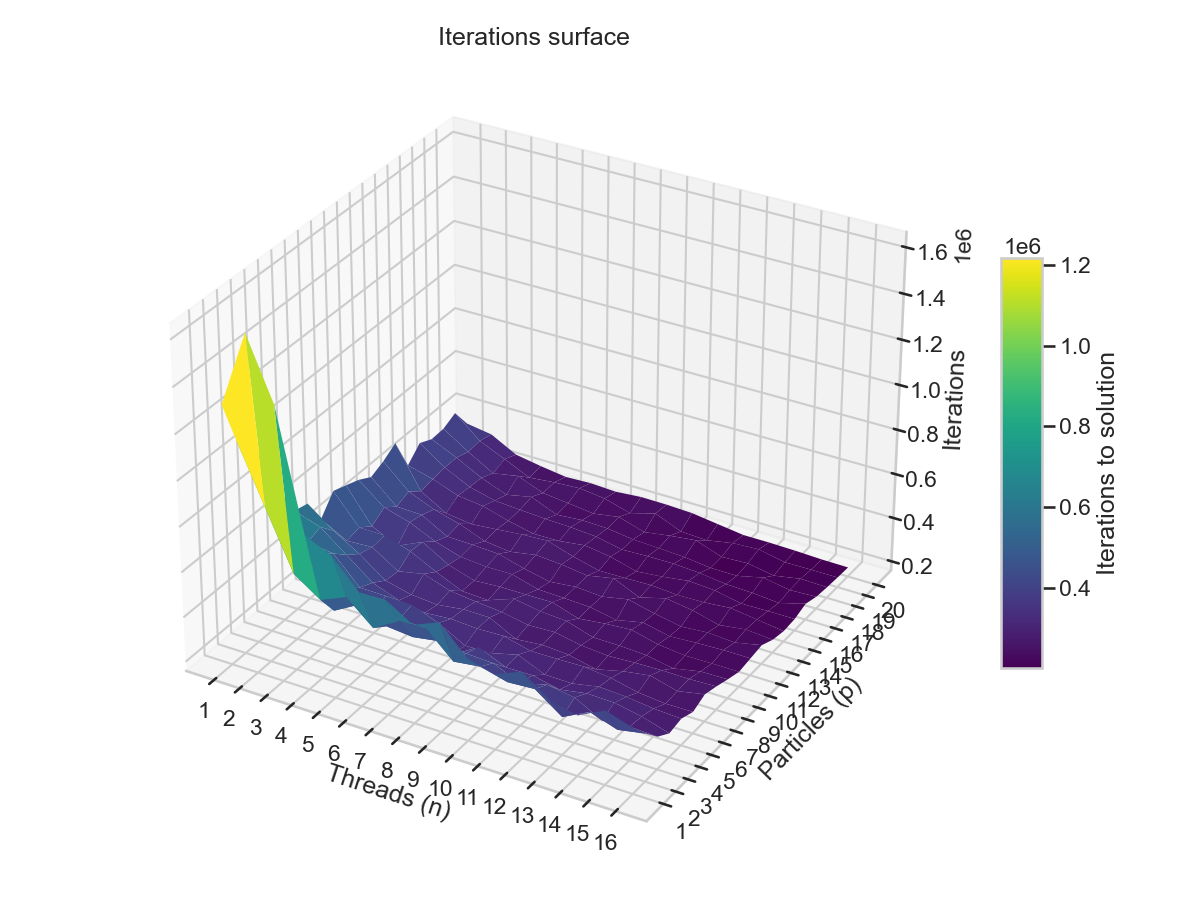
\includegraphics[width=0.8\textwidth]{Graphs/Graph Mesh Iters.png}
    \caption{Grafico mesh del numero di iterazioni/step del percorso trovato al variare del numero di thread e del numero di particelle per thread}
    \label{fig:mesh_iters}
\end{figure}

Dal grafico si nota come il numero di step del percorso trovato dopo la ricerca diminuisca notevolmente all'aumentare del numero di particelle. Anche l'aumento dei thread aumenta il numero di particelle totale: $p_{tot}=p*n$. \\
\noindent Questo conferma l'ipotesi teorica in cui avere più particelle aumenta la probabilità di trovare un percorso migliore, infatti le iterazioni sembrano seguire una decrescita proporzionale a $1/P_{tot}$.


\subsubsection{Speedup rispetto alla singola particella}

\begin{figure}[H]
    \centering
    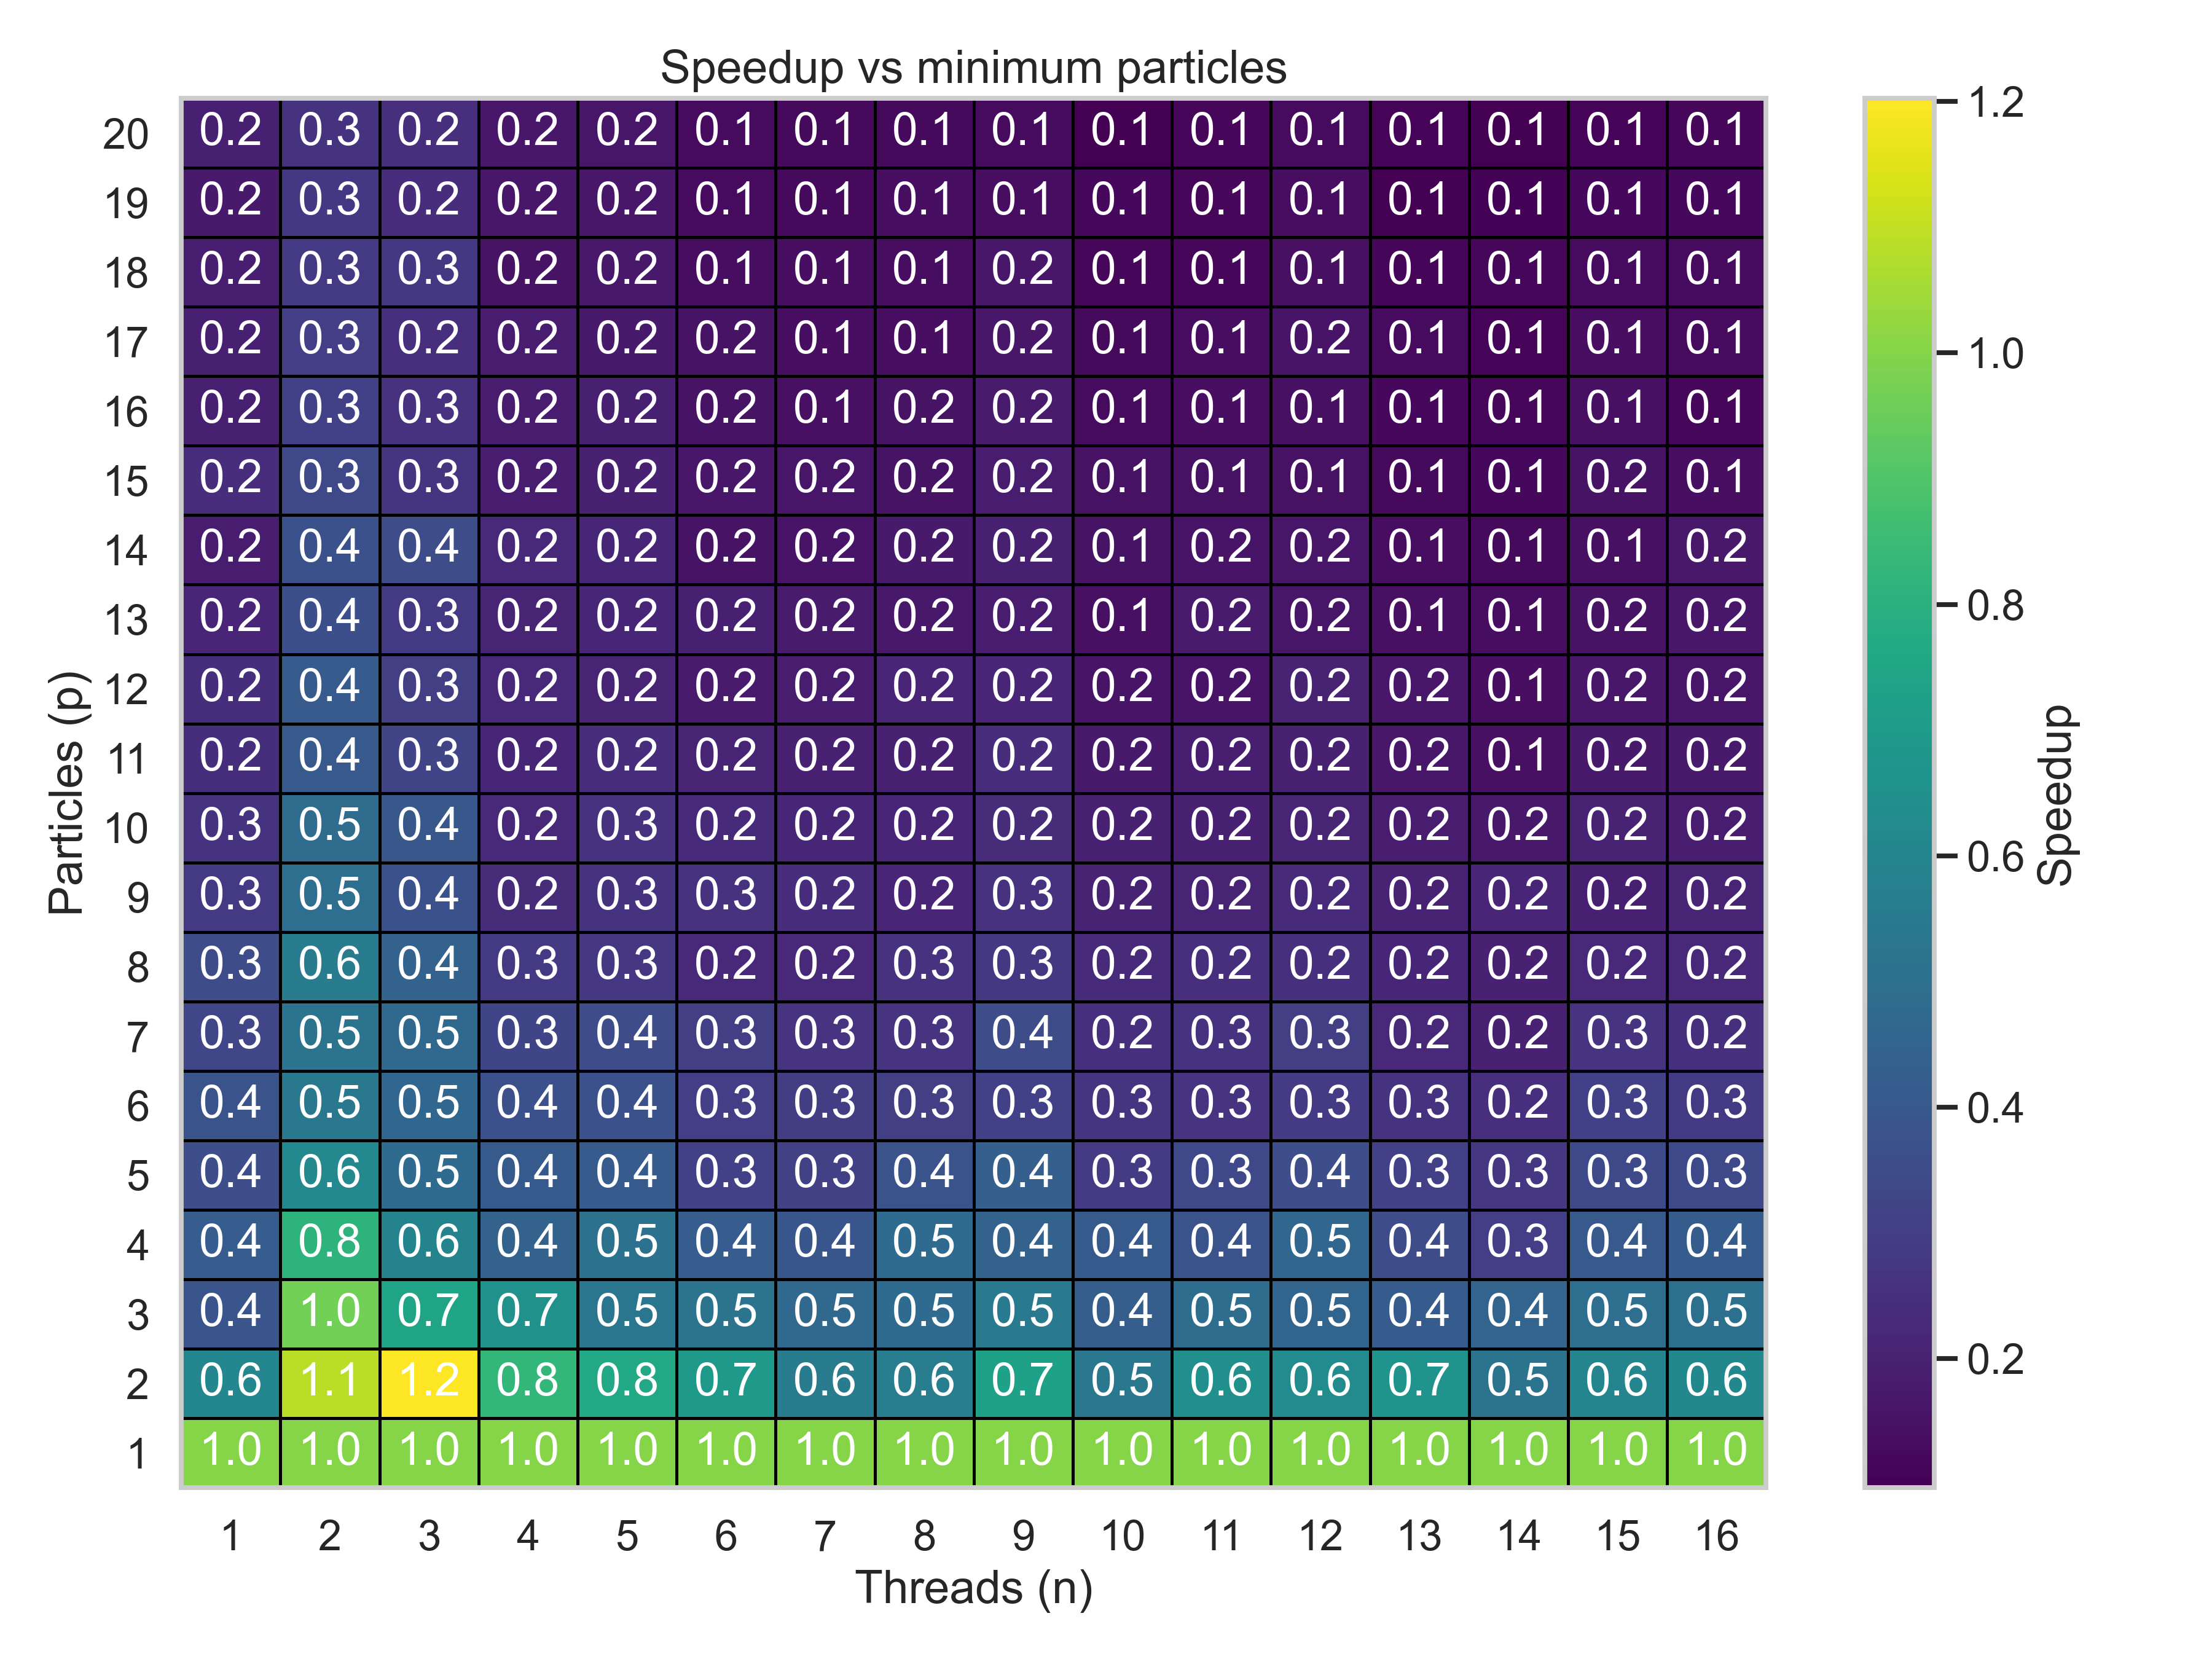
\includegraphics[width=0.8\textwidth]{Graphs/Heatmap Speedup 1-n.png}
    \caption{Heatmap dello speedup, calcolato rispetto a $T(1,n)$}
    \label{fig:heatmap_speedup_1_n}
\end{figure}

\noindent Formula: $S(p,n) = T(1,n)/T(p,n)$\\
\noindent Questa metrica permette di valutare l'effetto della variazione del numero di particelle rispetto al numero di thread $n$ fissato. Aumentando il numero di particelle, il carico di lavoro del thread aumenta linearmente, quindi se generalmente per arrivare alla soluzione un thread impiega (in media) $x$ step di una particella, con $n$ particelle dovrà eseguire $n*x$ iterazioni totali.\\
È vero che un numero di particelle maggiore aumenta la probabilità di trovare un cammino più veloce, ma non compensa a sufficienza il costo del carico aggiuntivo, però giustifica la decrescita non lineare dello speedup (fissato $n$).\\
\noindent Valori come $S(2,3)=1.2$ sono da considerarsi anomalie di misurazione dovute alla grande varianza dei dati a causa della componente random alla base (vedi \ref{subsec:difficulties}).


\subsubsection{Speedup rispetto al singolo thread}
\label{subsubsec:speedup_p_1}

\begin{figure}[H]
    \centering
    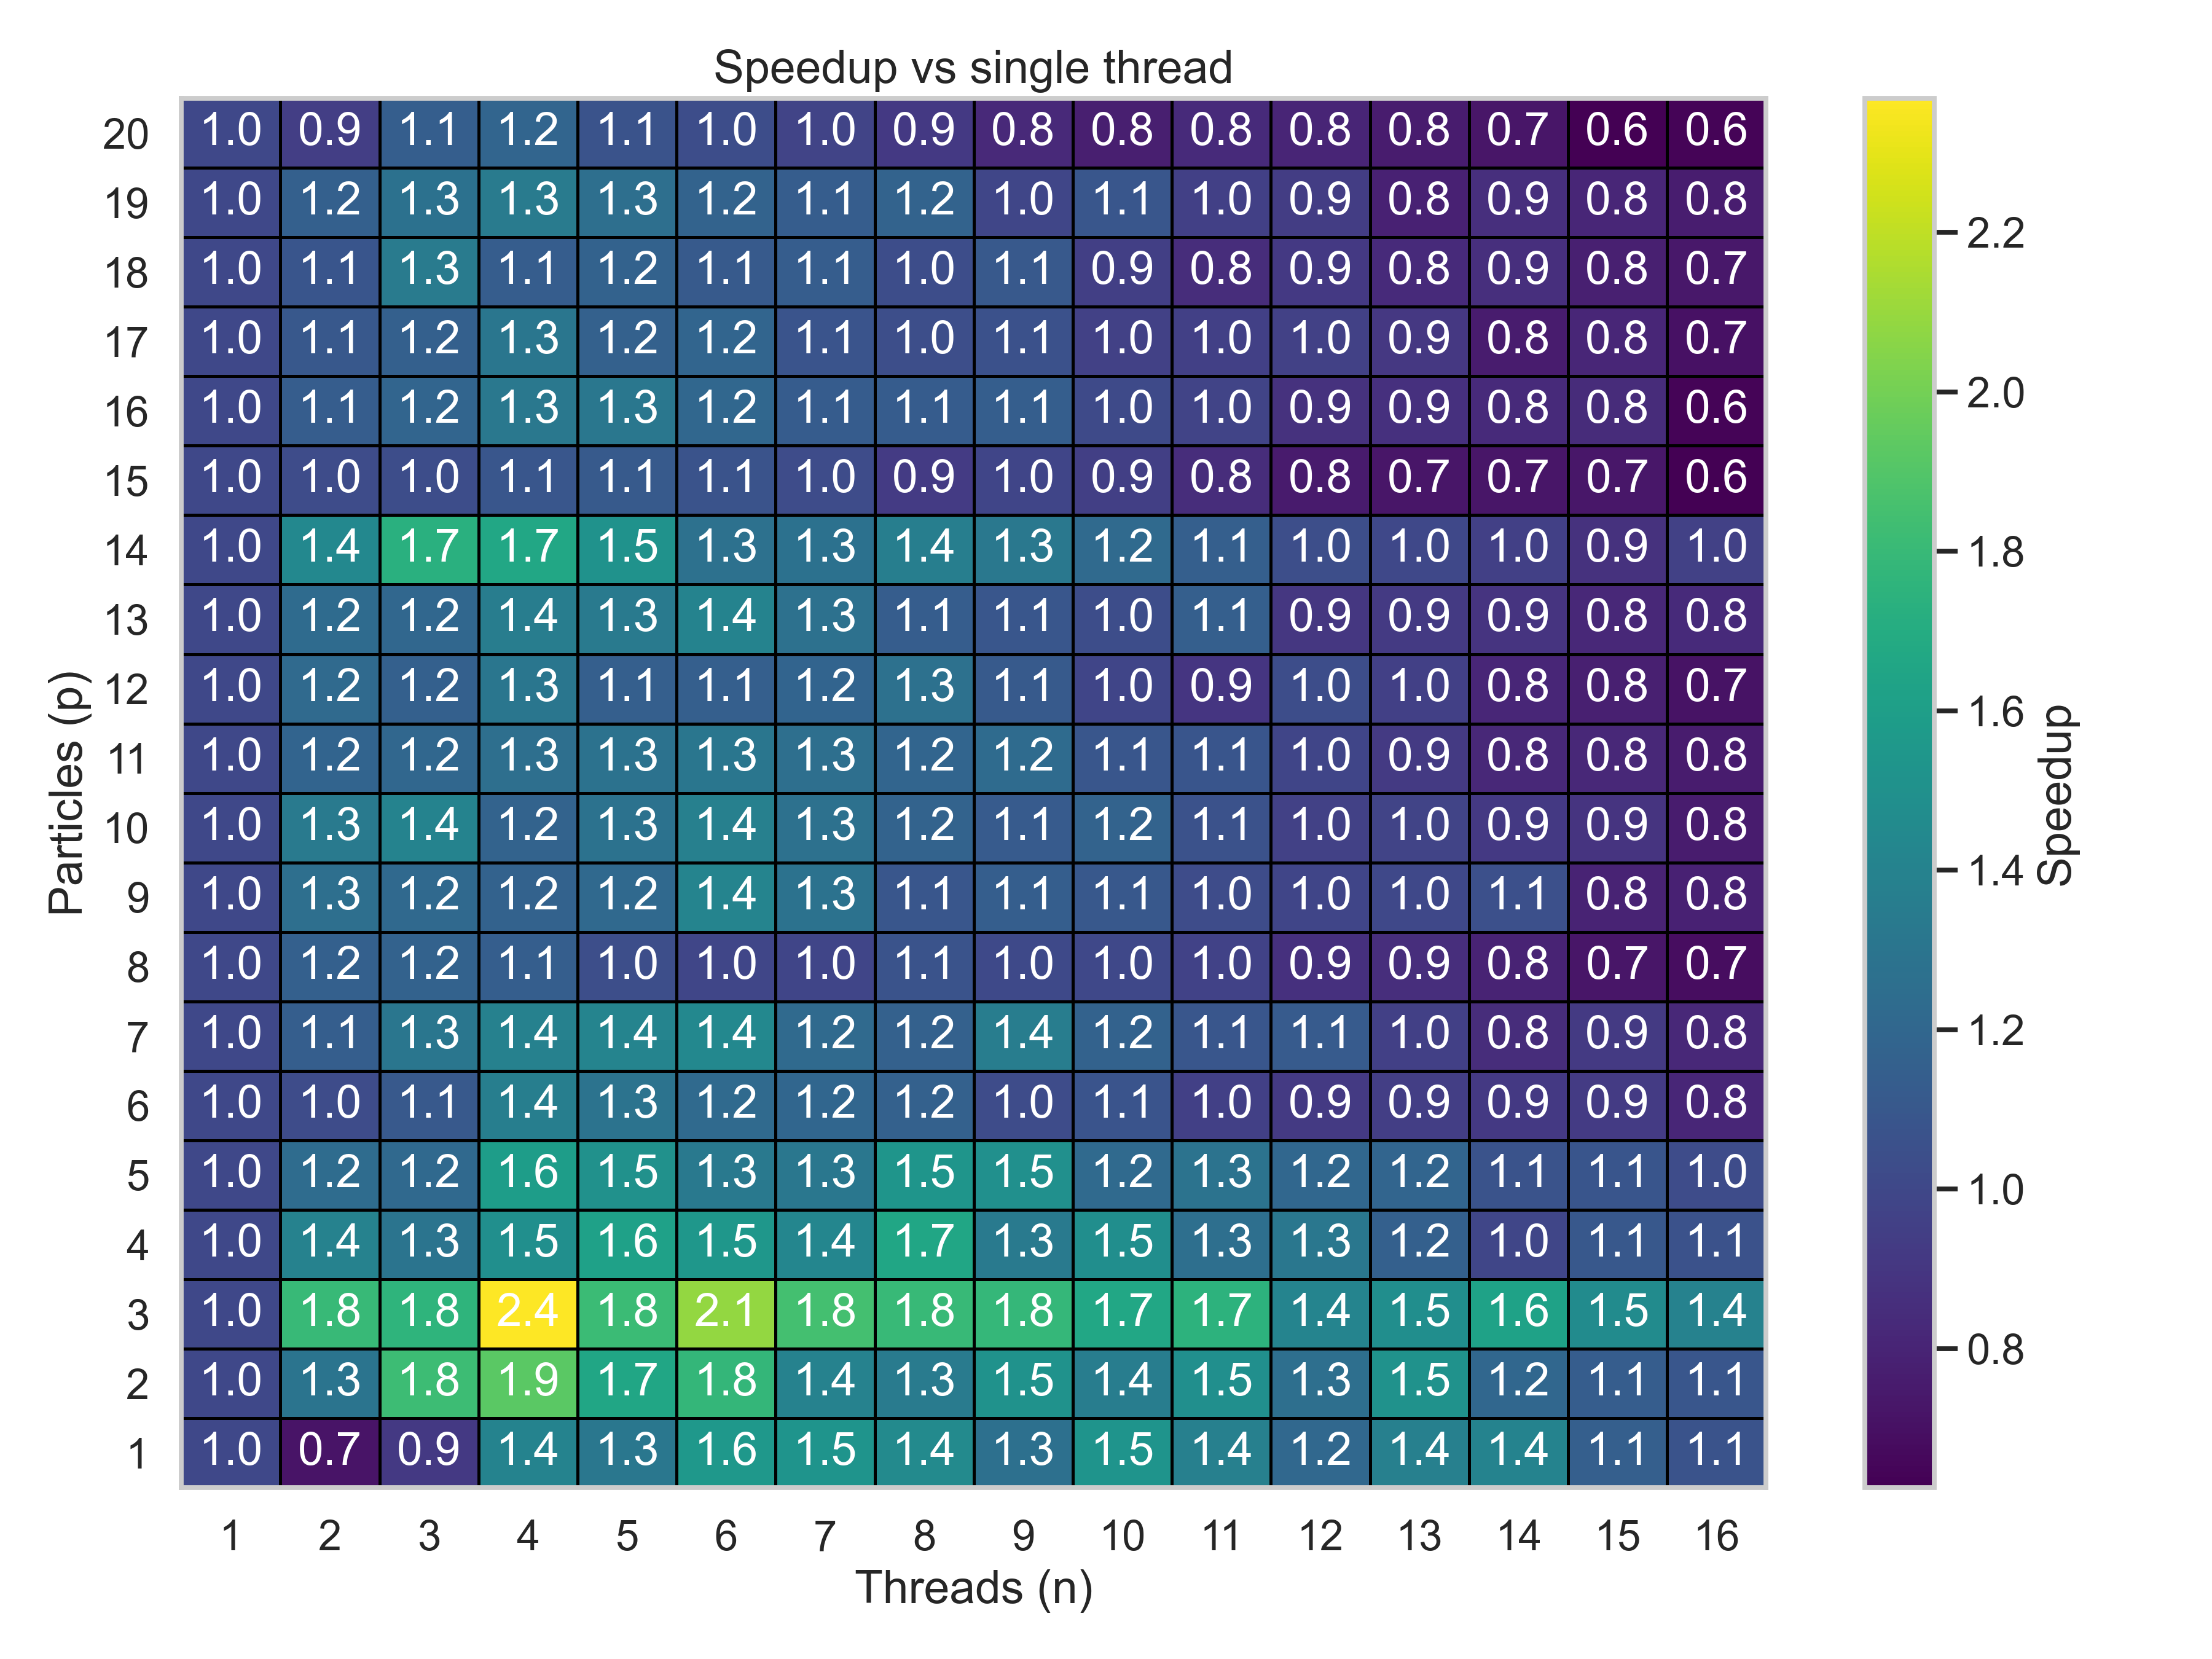
\includegraphics[width=0.8\textwidth]{Graphs/Heatmap Speedup p-1.png}
    \caption{Heatmap dello speedup, calcolato rispetto a $T(p,1)$}
    \label{fig:heatmap_speedup_p_1}
\end{figure}

\noindent Formula: $S(p,n) = T(p,1)/T(p,n)$\\
\noindent Valutando lo speedup relativo all'introduzione di ulteriori thread nella ricerca, è evidente che si ottiene un beneficio: avere più agenti che agiscono quindi su nuove particelle, aumenta la probabilità di trovare un percorso alla destinazione più breve. Questo miglioramento è praticamente gratuito finché ci sono core fisici disponibili nella CPU.\\
\noindent L'unico costo aggiuntivo è quello di creazione, gestione e sincronizzazione dei thread (assente del tutto solo nel caso in cui $n=1$): per questo motivo, come si vede dalla heatmap, avere 1 particella per thread con soltanto 2 thread, non rende giustizia a questo costo aggiuntivo e si ottiene di fatto un peggioramento delle prestazioni.
\noindent In generale i valori massimi di speedup si raggiungono con un numero di thread da $6$ a $8$, dopodiché i valori tornano a scendere. Questo comportamento è coerente con l'architettura della CPU utilizzata, che offre 8 core fisici e 16 thread logici (SMT): fino a $n=8$ ogni thread ha a disposizione un core fisico dedicato, e il guadagno di parallelizzazione è reale. Superato questo limite, i thread aggiuntivi condividono le cache L1/L2 dello stesso core fisico tramite SMT, che genera quindi situazioni di contesa.

\newpage

\subsubsection{Speedup complessivo}
$S(p,n) = T(1,1)/T(p,n)$.

\begin{figure}[H]
    \centering
    \begin{minipage}{0.49\textwidth}
        \centering
        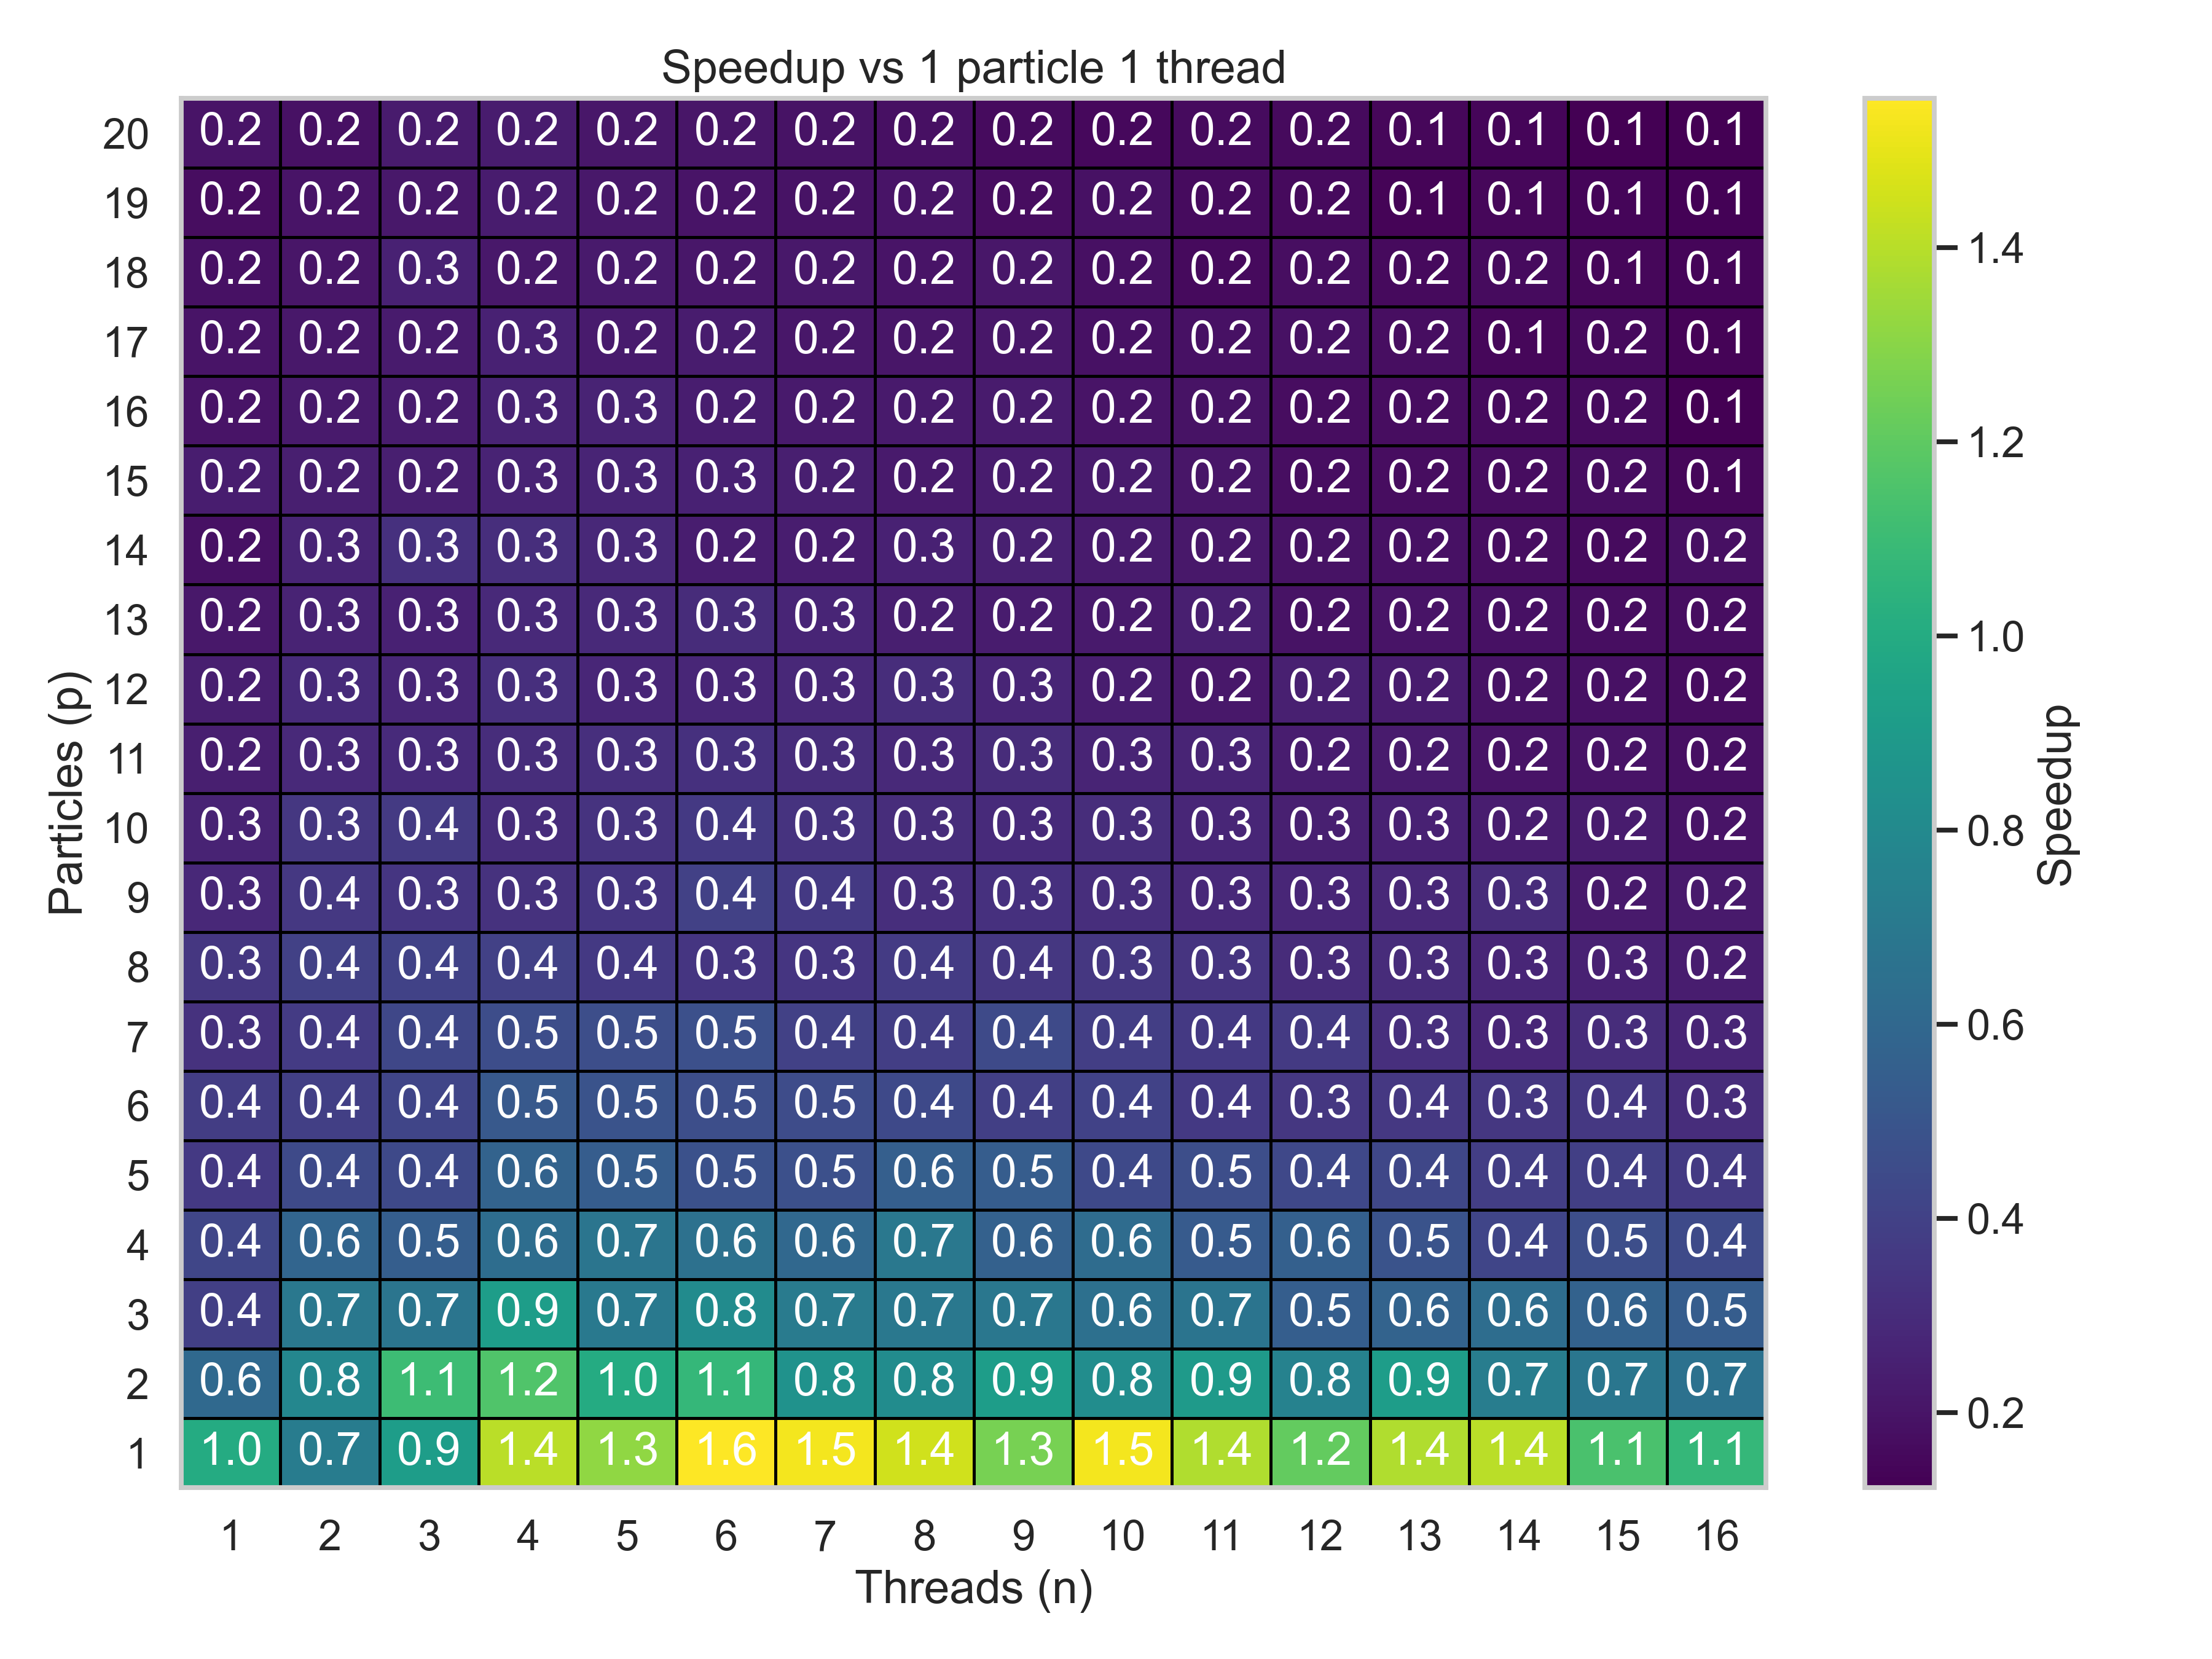
\includegraphics[width=\textwidth]{Graphs/Heatmap Speedup 1-1.png}
        \caption{Heatmap dello speedup, calcolato rispetto a $T(1,1)$}
        \label{fig:heatmap_speedup_1_1}
    \end{minipage}
    \begin{minipage}{0.49\textwidth}
        \centering
        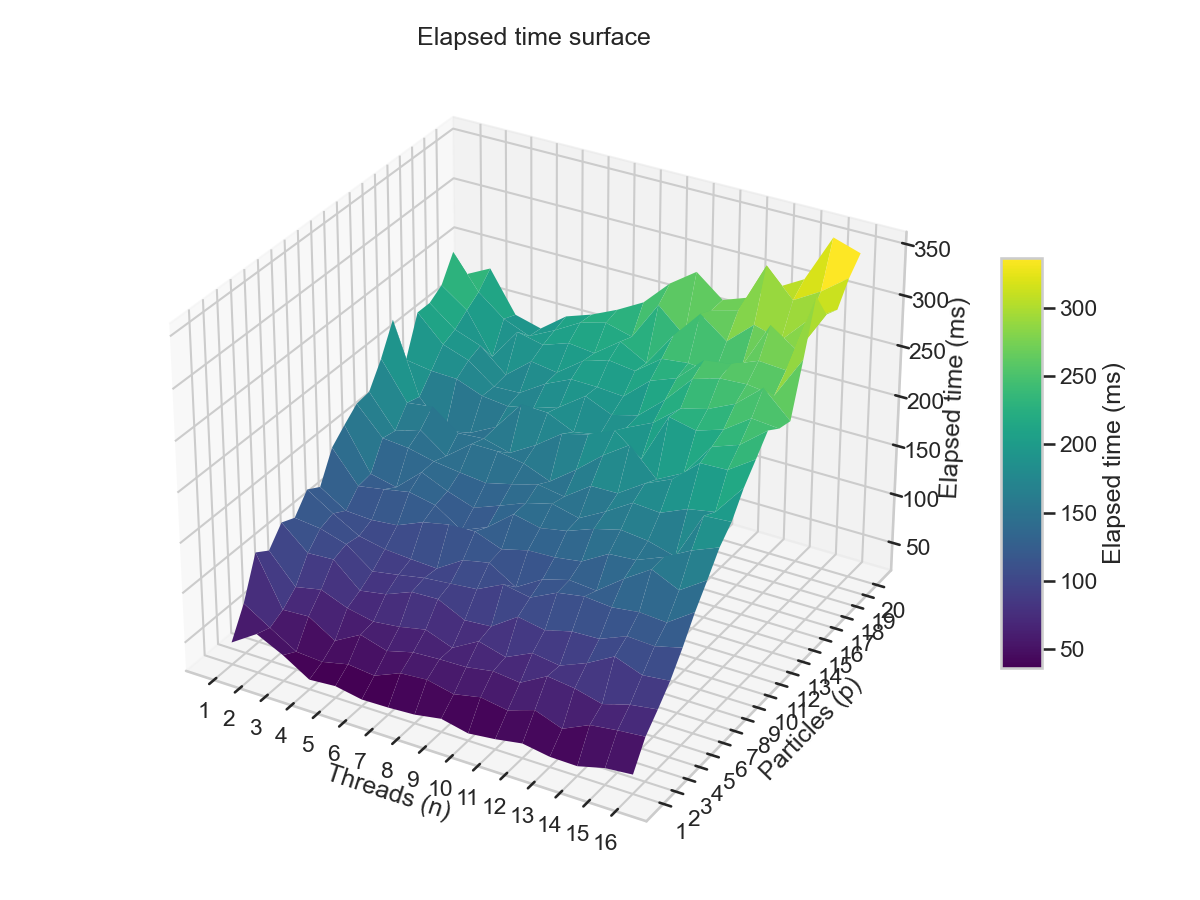
\includegraphics[width=\textwidth]{Graphs/Graph Mesh Time.png}
        \caption{Grafico mesh dei tempi misurati}
        \label{fig:mesh_time}
    \end{minipage}
\end{figure}


\noindent Formula: $S(p,n) = T(1,1)/T(p,n)$\\
\noindent L'heatmap qui sopra mostra lo speedup netto rispetto al caso base (1 particella, 1 thread). Da questo è possibile notare il peso reale dell'aumento del numero delle particelle piuttosto che quello di thread: a livello di prestazioni è molto più conveniente aggiungere nuovi thread, che lavorano comunque su un numero limitato di particelle, piuttosto che avere molte particelle su pochi thread.\\
\noindent Nel grafico dei tempi si nota come il tempo assoluto richiesto aumenti sia con $p$ che con $n$.
\noindent Nuovamente i valori di picco si trovano per valori di thread intorno a 8, per i motivi spiegati nella sezione \ref{subsubsec:speedup_p_1}.

\section{Conclusioni}
Visti i risultati ottenuti, è possibile concludere che:
\begin{itemize}
    \item l'elevata variabilità intrinseca del problema rende molto difficile studiarne le prestazioni.
    \item aumentare il numero di particelle riduce fortemente il numero di step del percorso finale trovato;
    \item aumentare il numero di thread produce uno speedup reale, che però si degrada superato il numero di thread fisici della macchina;
\end{itemize}
\noindent Pertanto la configurazione ottimale per questo algoritmo, con un buon compromesso tra lunghezza del percorso e tempi di esecuzione, si trova con un numero basso di particelle per thread ($p=4$) e un numero di thread entro pari ai core fisici disponibili ($n=8$ sulla CPU utilizzata).

\end{document}
